\documentclass{standalone}

\usepackage{graphics}
\usepackage[dvipsnames,svgnames]{xcolor}

\usepackage{tikz,pgf,pgfplots,circuitikz}
\pgfplotsset{compat=1.15}
\usetikzlibrary{shapes.symbols,intersections,arrows.meta,angles,calc,3d,decorations.pathmorphing}
\usepackage[compat=1.1.0]{tikz-feynhand}

\usepackage{amssymb,amsfonts,amsthm,mathtools}
\usepackage{physics,braket,bm}

\begin{document}  
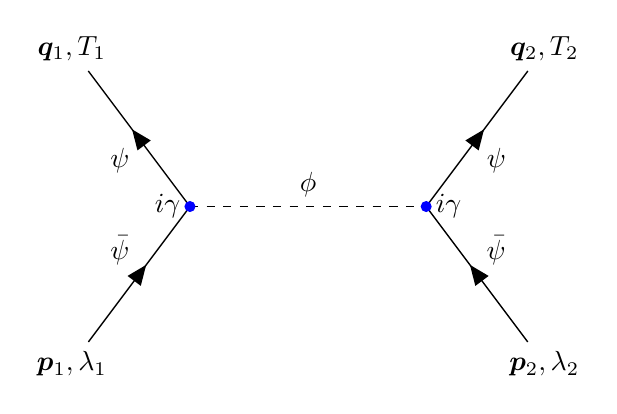
\begin{tikzpicture}
    \begin{feynhand}
        % Incoming fermions
        \vertex (i1) at (-3,2) {$\bm{q}_1, T_1$};
        \vertex (i2) at (-3,-2) {$\bm{p}_1, \lambda_1$};
        \vertex (o1) at (3,2) {$\bm{q}_2, T_2$};
        \vertex (o2) at (3,-2) {$\bm{p}_2, \lambda_2$};
        \vertex (v1) at (-1.5,0);
        \vertex (v2) at (+1.5,0);

        \propag[fer] (v1) to [edge label=$\psi$] (i1);
        \propag[fer] (i2) to [edge label=$\bar{\psi}$] (v1);
        \propag[fer] (v2) to [edge label'=$\psi$] (o1);
        \propag[fer] (o2) to [edge label'=$\bar{\psi}$] (v2);        
        
        \propag[sca] (v1) to [edge label=$\phi$] (v2);

        \fill[blue] (v1) circle (2pt) node [left, black] {$i\gamma$};
        \fill[blue] (v2) circle (2pt) node [right, black] {$i\gamma$};
    \end{feynhand}
\end{tikzpicture}
\end{document}
